\chapter{Introduction}

Each year, the robotic community gathers at conferences such as IROS
(International Conference on Intelligent Robots and Systems), where they
exhibit their discoveries and achievements in the field. For the year 2019, the
Drone Racing League will be hosting a series of races which autonomous drones
will compete and attempt to outperform a professional drone pilot.\\

\begin{figure}[h]
	\centering
	\includegraphics[width=0.5\textwidth]{figure/iros_2016.jpg}
	\caption{Drone racing arena at IROS 2016.}
	\label{fig:iros}
\end{figure}

The company Lockheed Martin is sponsoring the event and offering a prize of 2
million USD for the winning team. Teams of university students and other drone
enthusiasts shall present innovative approaches on vision-based systems for
unmanned aerial vehicles: hence, they showcase their progress through racing.\\

\section{What is drone racing?}

As in any race, competitors measure their skills at maneuvering their vehicle,
from within or at distance, against the clock or against themselves, in an
attempt to complete a circuit before everyone else.

In drone racing, the circuit is comprised of a set of obstacles, static or
dynamic, usually arranged in a loop. For the case of classic drone racing, huge
futuristic-looking arenas are used as a playground for extremely skilled pilots,
who make the race look impressive and dynamic by the use of FPV goggles to fly
the drones at very high speed, reaching 120mph
\cite{https://thedroneracingleague.com/learn-more/}.

\begin{figure}[h]
	\centering
	\includegraphics[width=0.5\textwidth]{figure/drl_arena.jpg}
	\caption{Drone Racing League arena in London (Steven Paston/PA)}
\end{figure}

\todo{cite image https://home.bt.com/tech-gadgets/tech-news/the-drone-racing-league-has-set-a-new-world-record-for-the-fastest-drone-around-11364196881110}
	
For the case of autonomous drone racing, up until the \emph{Drone Racing
League} announced their autonomous competition of 2019, arenas looked much more
like a laboratory than a glowing circuit, as it can be seen on Figure
~\ref{fig:mygates} showing the AiR Lab in Skejby (Aarhus, DK), with its gates
built and painted for this work. These obstacles were inspired of the previous
competitions organized by IROS, as seen on Figure ~\ref{fig:iros} which also
shows the typical type of drones used in this research area: consumer drones
for the larger audience. This kind of drones is not made for sportive flight,
but mostly for an easy hands-on experience, providing a relatively slow but
stable flight.

\begin{figure}[h]
	\centering
	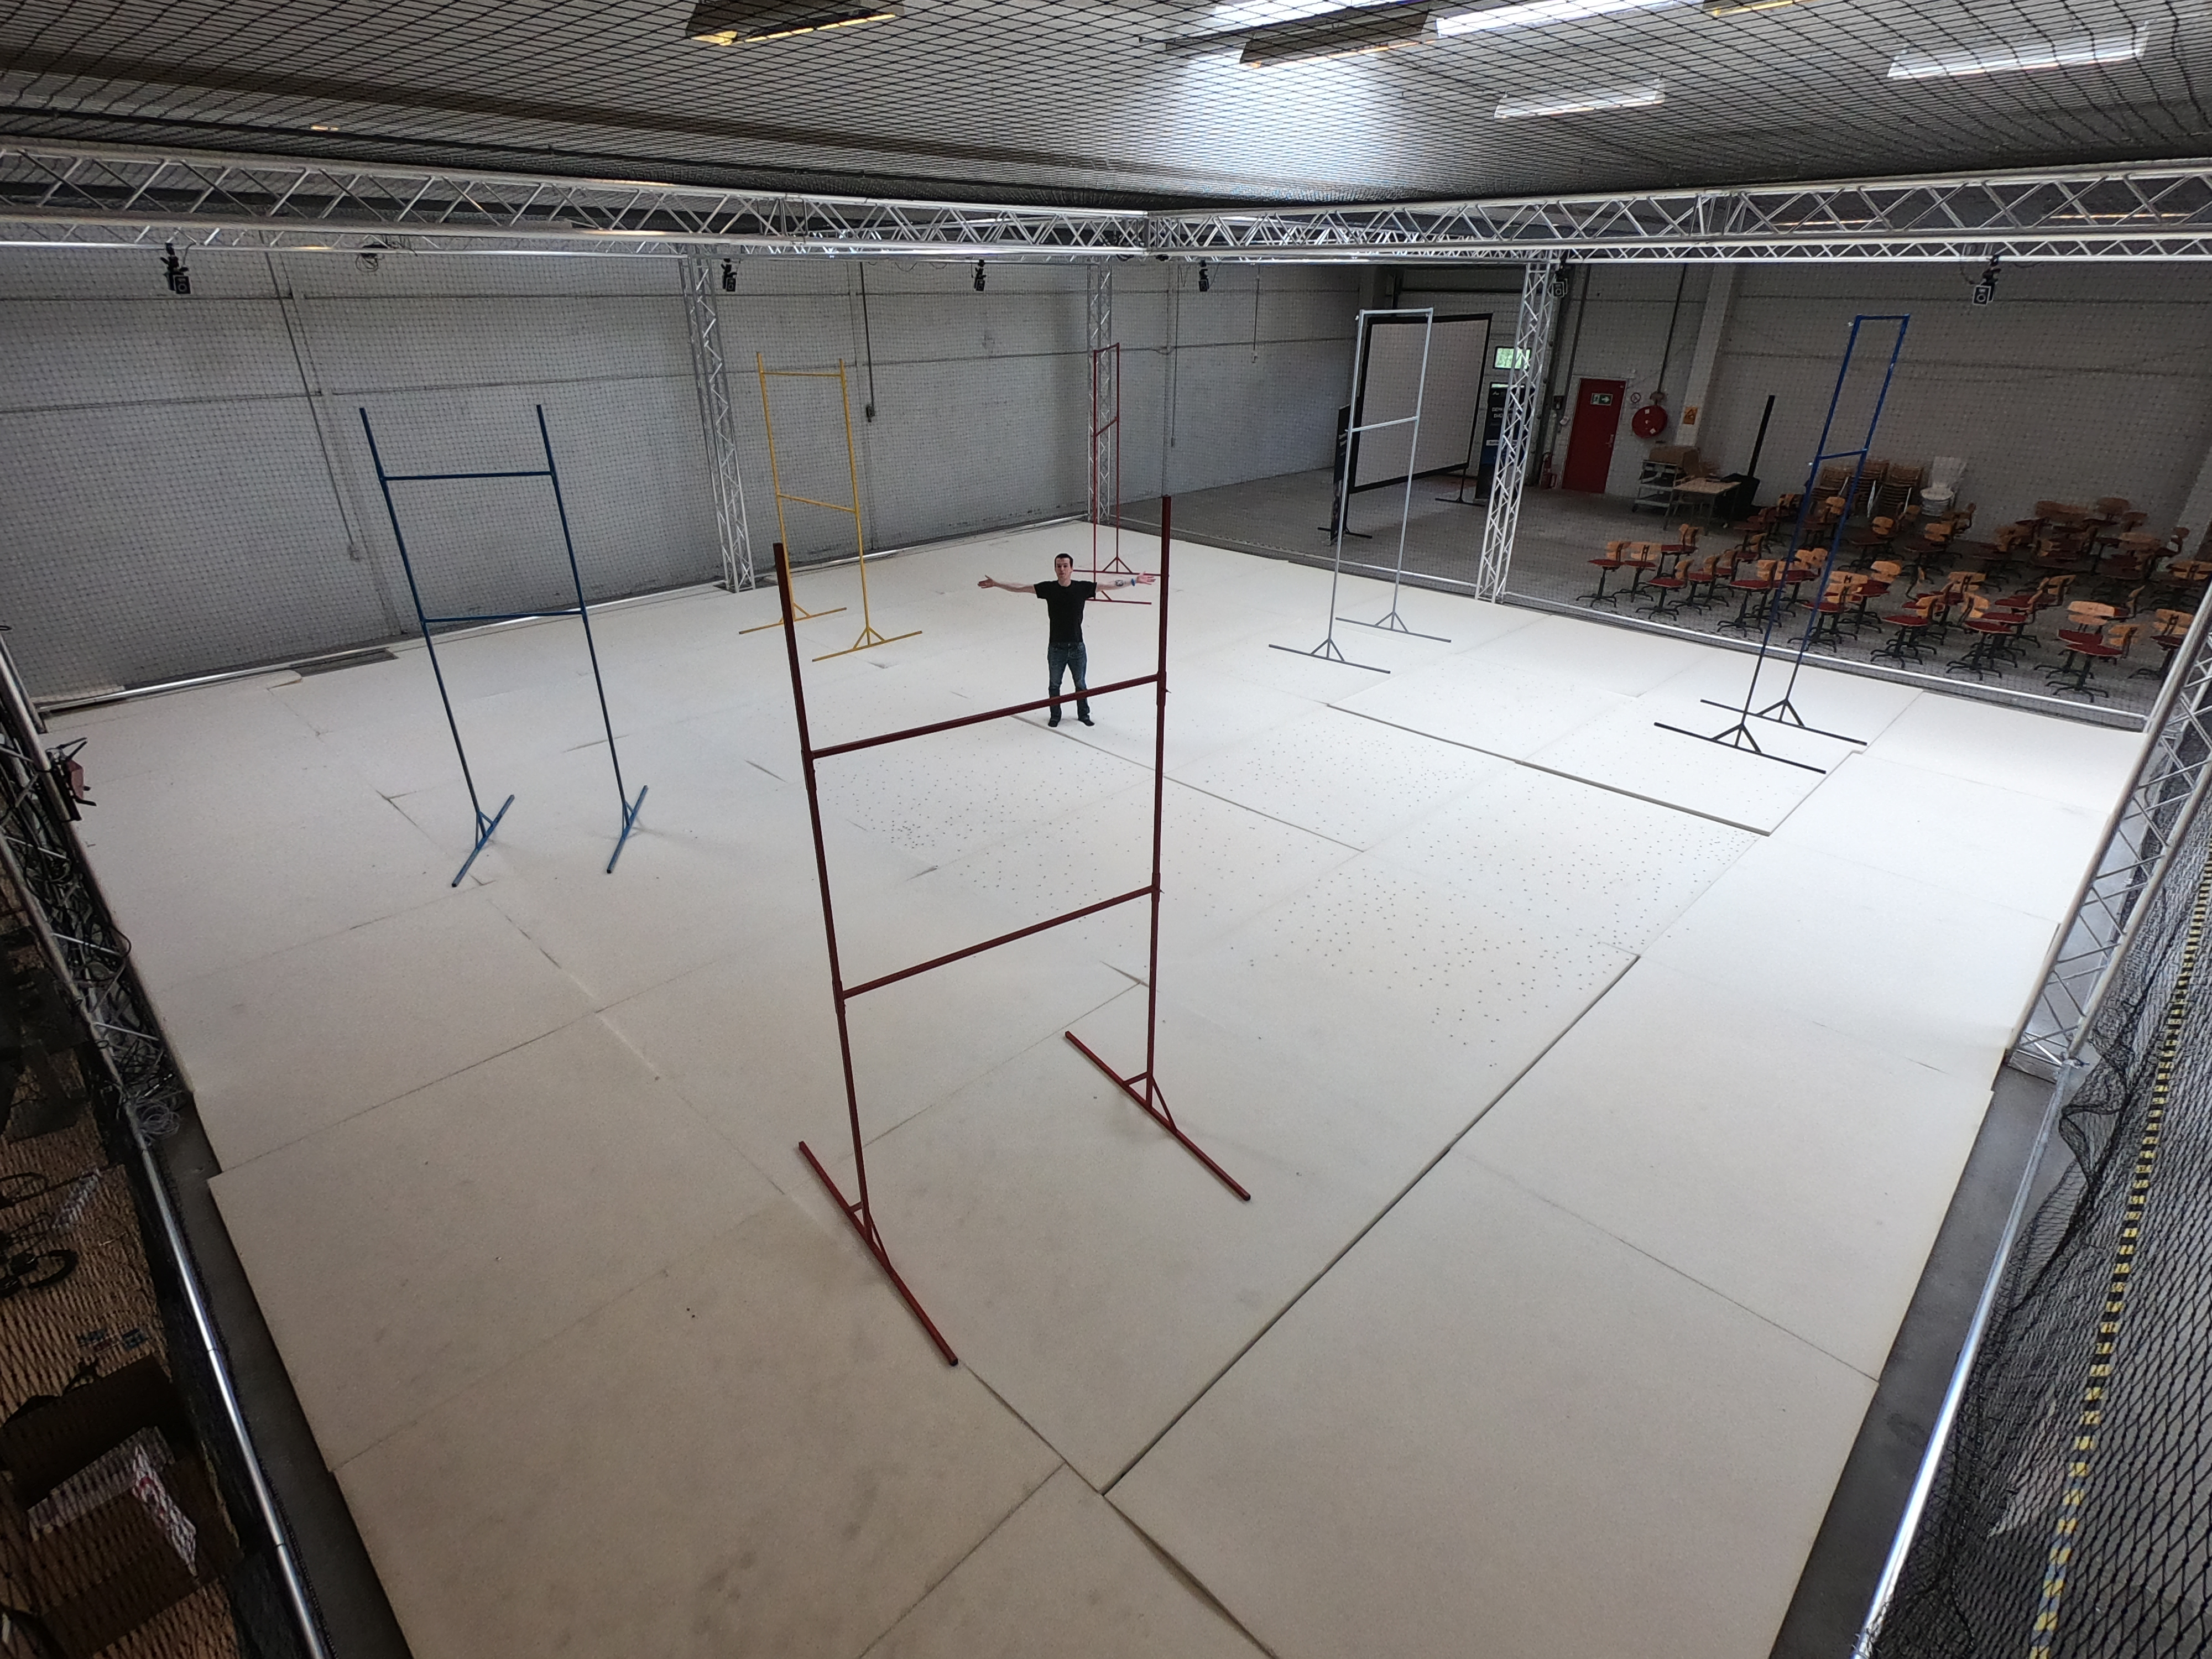
\includegraphics[width=0.5\textwidth]{figure/tiny_me.jpg}
	\caption{The AiR Lab and the custom built obstacles around the author in Skejby}
	\label{fig:mygates}
\end{figure}

The goal is to complete a given amount of turns as fast as possible, but since
it is still the early days of drone racing and the costs of a potential crash
would be too high, each drone races against the clock, one after an other.
Ultimately, autonomous drones will be racing against skilled pilots, as the
\emph{Drone Racing League} seems to encourage it by giving a total prize of 2
millions USD for the race of 2019.


\subsection{Stakes}
\todo{Talk about the predictions for AI in drone racing and drones in general
for the future}


\subsection{Beyond the hype and into reality}
\todo{Talk about Amazon Prime Air, food delivery, driverless taxis...}


\subsection{Challenges}
Most robotic system's operation can be modeled by the commonly known
\emph{Sense, Plan, Act} paradigm:
\todo{Add custom act, sense, plan paradigm picture}
\begin{figure}[h]
	\centering
	\includegraphics[width=0.4\textwidth]{figure/robotic_paradigm.png}
	\caption{The Sense, Plan, Act robotic paradigm.}
	\label{fig:robotic_paradigm}
\end{figure}

\begin{itemize}
	\item{\textbf{Sense}}: gather information using sensors (camera, IMU, sonar...).
	\item{\textbf{Plan}}:create a world model using all the information, and plan
		the nextmove.
	\item{\textbf{Act}}: carry out the actions that the plan calls for.
\end{itemize}
~\\
This thesis will be focused mainly on the sensing of the drone control, and
more precisely using computer vision algorithms along with machine learning
concepts. However, an important part of the trajectory planning directly
follows the sensing phase, therefore those two first phases of the control loop
can be included in the scope of the project.

To this day, most drones in the robotic research field are running \emph{Robot
Operating System} (ROS) \todo{Add citation}, which is a set of "libraries and
tools to help software developers create robot applications". The implementation
of the computer vision algorithms will be constrained within ROS, and cooperate
with the different control components provided by the project team.\\





\section{Litterature review}

\subsection{The modern approach}
Most robotic system's operation can be modeled by the commonly known
\emph{Sense, Plan, Act} paradigm:
\todo{Add custom act, sense, plan paradigm picture}
\begin{figure}[h]
	\centering
	\includegraphics[width=0.4\textwidth]{figure/robotic_paradigm.png}
	\caption{The Sense, Plan, Act robotic paradigm.}
	\label{fig:robotic_paradigm}
\end{figure}

\begin{itemize}
	\item{\textbf{Sense}}: gather information using sensors (camera, IMU, sonar...).
	\item{\textbf{Plan}}:create a world model using all the information, and plan
		the nextmove.
	\item{\textbf{Act}}: carry out the actions that the plan calls for.
\end{itemize}
~\\
This thesis will be focused mainly on the sensing of the drone control, and
more precisely using computer vision algorithms along with machine learning
concepts. However, an important part of the trajectory planning directly
follows the sensing phase, therefore those two first phases of the control loop
can be included in the scope of the project.

To this day, most drones in the robotic research field are running \emph{Robot
Operating System} (ROS) \todo{Add citation}, which is a set of "libraries and
tools to help software developers create robot applications". The implementation
of the computer vision algorithms will be constrained within ROS, and cooperate
with the different control components provided by the project team.\\

\todo{Talk about why CNNs are used more and more in drone racing, and basically
why it is the chosen approach, which leads to tackling the dataset generation
problem.}

As Deep Learning has known an exponential growth during the past decade,
computer vision applications tend to exploit the power of convolutional neural
networks more and more. Thanks to their impressive accuracy in specific problem
solving, CNNs are becoming the main choice for tasks such as: object detection,
object segmentation, object recognition, \emph{etc}\ldots

In drone racing, the latest works, which are often the best performing, tend to
employ CNNs for the sensing part, or even as an all-in-one solution.\\


\section{The chosen approach}

In order to make things easier and to be able to set tangible milestones, the
challenge is split in two logical problems to be solved, one after the
other. The problem is not solved as a whole race, but rather as a trajectory
between a starting point and a gate. This choice of approach is motivated by
the fact that admitedly, if the nearest gate detection is quick and precise,
considering a race as a succession of independent targets to be reached is
theoreticaly a robust solution that can be applied to any environment, with any
obstacles, and of any length.\\

\begin{figure}[h]
	\centering
	\includegraphics[width=0.5\textwidth]{figure/300x300.png}
	\caption{System diagram.}
	\label{fig:iros}
\end{figure}

Firstly, the perception logic is solved with a deep learning algorithm, most
precisely with a convolutional neural network. However, it has been seen from
the literature review that collecting a dataset for drone racing can be
tedious, and is rarely variate enough to allow for good generalization of the
learning and application in any given environment. In this work, a
semi-synthetic dataset is generated from background images, to provide an
infinite amount of circuit combinations to train the gate recognition network
(more on that in the following chapter).

Being the main research topic of this thesis, this part is given more time and
focus to deliver a more rigourous and in-depth work.\\

\begin{figure}[h]
	\centering
	\includegraphics[width=0.5\textwidth]{figure/300x300.png}
	\caption{Block diagram of the perception logic.}
	\label{fig:iros}
\end{figure}

Secondly, the control logic is made as simple as can be, since its purpose is
only to verify the hypothesis proposed for the perception. A state machine is
supervising the flight between the two gates, and utilizes a
Proportional-Integral-Derivative controller to output velocity commands to the
lower-level controller implemented by the manufacturer on the UAV.\\

\begin{figure}[h]
	\centering
	\includegraphics[width=0.5\textwidth]{figure/300x300.png}
	\caption{Block diagram of the control logic.}
	\label{fig:iros}
\end{figure}


As for the drone itself, 

The solution will be implemented iteratively, by gradually increasing the
complexity of the vision algorithms, such that progress can be made even if the
end goal is too difficult to achieve.\\

The project should attempt to fulfill the following goals:

\begin{itemize}
	\item{Recognize gates in the input image}
	\item{Detect and localize the closest gate's center}
	\item{Evaluate the closest gate's orientation and distance}
	\item{Plan a trajectory for the drone to fly across the gate center}
	\item{Refine the trajectory in real time, for an optimal flight time}
	\item{Make the drone follow that trajectory while adjusting in real time}
\end{itemize}
~\\
However, the following functionalities are out of the scope and will be
discarded:

\begin{itemize}
	\item{Detect any other obstacles in the input image}
	\item{Avoid obstacles that are on the drone's trajectory}
	\item{Map and localize the detected gates in world frame}
	\item{Plan a trajectory of a sequence of gates}
	\item{Apply online learning for adaptive racing}
\end{itemize}


\todo{System diagram, framework, ROS and all the shit}

